\chapter{Généralité sur les systèmes photovoltaïques et les batteries solaires}
\phantomsection
%\addcontentsline{toc}{chapter}{Batterie} 
\section{Introduction}
L’énergie photovoltaïque représente une solution prometteuse pour réduire notre dépendance aux formes d’énergie traditionnelles, souvent sources de pollution et non renouvelables. Malgré ses avantages, elle présente certains inconvénients, notamment un faible rendement des matériaux de conversion, une maîtrise insuffisante des systèmes de stockage, et des coûts encore élevés par rapport à d’autres formes d’énergie   .

Cette étude explore l'impact et les avantages de l'énergie photovoltaïque en examinant ses domaines d'application, les sous-systèmes essentiels comme les batteries solaires, et les méthodes de dimensionnement des installations photovoltaïques. 

\section{Les applications photovoltaïques}
Les applications photovoltaïques terrestres se divisent en trois types \cite{t1} :
\begin{itemize}
	\item \textbf{Systèmes autonomes} : utilisent uniquement l’énergie solaire, avec des accumulateurs pour stocker l’énergie, ou fonctionnent sans batteries pour des applications comme le pompage de l’eau.
	\item \textbf{Systèmes hybrides} : combinent des panneaux photovoltaïques avec une éolienne ou un groupe électrogène pour une alimentation continue et de haute puissance, réduisant les besoins en panneaux solaires et batteries.
	\item \textbf{Systèmes connectés au réseau} : produisent de l’énergie localement et transfèrent l'excédent au réseau, sans batteries, bien qu'elles puissent être utilisées en secours.
\end{itemize}


D'autres domaines peuvent également tirer parti des technologies photovoltaïques, \\
tels que :
\begin{itemize}
	\item Systèmes embarqués (téléphones, netbooks, tablettes, etc.)
	\item Systèmes spatiaux.
\end{itemize}


\begin{figure}[H]
	\centering
	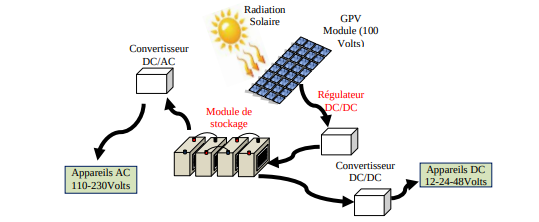
\includegraphics[width=14cm]{./img/standAlone.png}
	\caption{Schéma générale d’une installation PV autonome.}
	\label{i1}
\end{figure}

\begin{figure}[H]
	\centering
	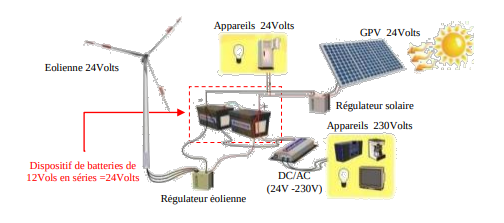
\includegraphics[width=14cm]{./img/hybrid.png}
	\caption{Schéma de raccordement d’une installation Hybride.}
	\label{i1}
\end{figure}


\section{Le panneau photovoltaïque}
Un panneau photovoltaïque est constitué de cellules solaires connectées électriquement en série et/ou en parallèle pour produire le courant et la tension souhaités.

\subsection{Cellule solaire}
La cellule photovoltaïque, fonctionnant grâce à l'effet photovoltaïque découvert par Becquerel en 1839, transforme l'énergie lumineuse en courant électrique via un matériau semi-conducteur, avec une tension d'environ 0,5 à 0,6 V \cite{l3}.\\

Il existe plusieurs types de cellules photovoltaïques :
\begin{itemize}
	\item \textbf{Cellule multi-jonction :} destinée aux applications spatiales, non commercialisée.
	\item \textbf{Cellule en silicium monocristallin :} formée à partir d’un seul cristal de silicium, bleu uniforme.
	\item \textbf{Cellule en silicium polycristallin :} composée de plusieurs cristaux, avec des motifs distincts.
	\item \textbf{Cellule en couche mince CIS/CIGS :} fabriquée à partir de cuivre-indium-sélénium ou gallium.
	\item \textbf{Cellule en silicium amorphe :} projette du silicium sur verre, couleur gris foncé ou marron.
	\item \textbf{Cellule CZTS :} produite avec des minerais non toxiques.
\end{itemize}

%\begin{figure}[H]
%	\centering
%	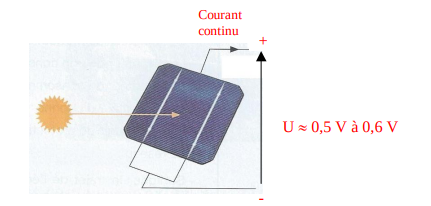
\includegraphics[width=5cm]{./img/cellule.png}
%	\caption{Exemple d'une cellule photovoltaïque}
%	\label{i1}
%\end{figure}
\subsubsection{Principe de fonctionnement}
Prenons le cas d'une cellule photovoltaïque fabriquée à partir de deux couches de silicium (matériau semi-conducteur) :
\begin{itemize}
	\item Une couche dopée avec du bore, qui possède moins d'électrons que le silicium, est dopée positivement (zone P).
	\item Une couche dopée avec du phosphore, qui possède plus d'électrons que le silicium, est dopée négativement (zone N).
\end{itemize}

\begin{figure}[H]
	\centering
	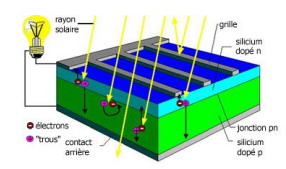
\includegraphics[width=8cm]{./img/cellulePrincipe.png}
	\caption{Détail d'une cellule photovoltaïque}
	\label{i1}
\end{figure}

Lorsqu'un photon de lumière arrive, son énergie crée une rupture entre un atome de silicium et un électron, modifiant les charges électriques. Les atomes, chargés positivement, migrent vers la zone P, tandis que les électrons, chargés négativement, se déplacent vers la zone N. Une différence de potentiel électrique, c'est-à-dire une tension électrique, est ainsi crée. C'est ce qu'on appelle l'effet photovoltaïque.

%\subsubsection{Association des cellules en série}

%Les caractéristiques d’une seule cellule photovoltaïque ne suffisent pas pour alimenter des équipements électriques. Les cellules sont donc associées en série pour obtenir une tension plus élevée, formant un module solaire ou panneau photovoltaïque de 9 ou 12 volts ... La puissance d’un panneau dépend de sa surface et du nombre de cellules qu'il contient.


%\begin{figure}[H]
%	\centering
%	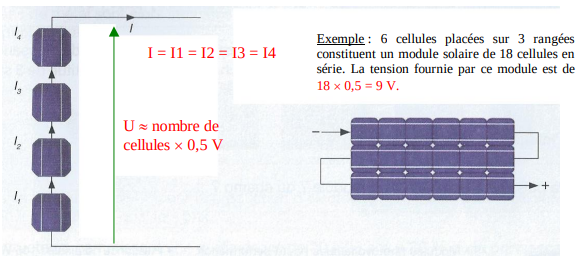
\includegraphics[width=15cm]{./img/exemple.png}
%	\caption{Exemple d'une association des cellules en série}
%	\label{i1}
%\end{figure}

%Pour faire fonctionner des appareils, l’intensité (I) du panneau, variant avec l’ensoleillement, détermine l’énergie produite. La puissance crête d’une installation, exprimée en watt-crête (Wc), est la puissance maximale fournie dans des conditions optimales d’orientation, d’inclinaison et d’ensoleillement.On peut trouver des variété de puissance d'un panneaux solaire comme 50, 100, 150, 200, 280, 300, 340 Wc , ... 

\subsubsection{Constitution d’un champ photovoltaïque}
Les panneaux solaires sont connectés en série pour obtenir la tension nécessaire à l'onduleur, formant une chaîne de modules ou "string". Les chaînes sont ensuite associées en parallèle pour constituer un champ photovoltaïque (champ PV). Des diodes ou des fusibles en série sur chaque chaîne protègent contre les courants inverses causés par l'ombre, évitant ainsi d'endommager les modules.\\

Il existe des differentes types de panneaux solaires :
\begin{itemize}
	\item Monocristallin
	\item Polycristallin
	\item Amorphe
	\item Multi-jonction
	\item CIS et CIGS
	\item CZTS
\end{itemize}
%\begin{figure}[H]
%	\centering
%	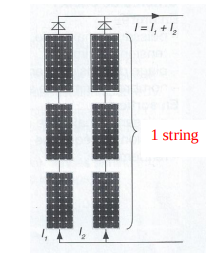
\includegraphics[width=6cm]{./img/string.png}
%	\caption{Chaîne de module ou "String"}
%	\label{i1}
%\end{figure}

%\subsection{Comparaison entre les différents types de panneaux solaires}

%Nous allons voir dans le tableau ci-dessous les différences entre les types de panneaux solaires selon leurs technologies de construction.

%\begin{table}[H]
%	\centering
%	\begin{tabular}{|>{\centering\arraybackslash}m{3cm}|>{\centering\arraybackslash}m{11cm}|>{\centering\arraybackslash}m{1.5cm}|}
%		\hline
%		\textbf{Technologie} & \textbf{Caractéristique} & \textbf{Part de marché} \\			
%		\hline
%		Monocristallin & \begin{itemize}
%			\item Très bon rendement : 14 à 20 \%.
%			\item Durée de vie : importante (30 ans).
%			\item Coût de fabrication : élevé.
%			\item Puissance : 100 à 150 Wc/m\textsuperscript{2}.
%%			\item Rendement faible sous un faible éclairement.
%			\item Perte de rendement avec l’élévation de la température.
%			\item Fabrication : élaborés à partir d’un bloc de silicium fondu qui s’est solidifié en formant un seul cristal.
%			\item Couleur bleue uniforme.
%		\end{itemize} & 43 \% \\
%		\hline
%		Polycristallin & \begin{itemize}
%			\item Bon rendement : 11 à 15 \%.
%			\item Durée de vie : importante (30 ans).
%			\item Coût de fabrication : meilleur marché que les panneaux monocristallins.
%			\item Puissance : 100 Wc/m\textsuperscript{2}.
%			\item Rendement faible sous un faible éclairement.
%			\item Perte de rendement avec l’élévation de la température.
%			\item Fabrication : élaborés à partir de silicium de qualité électronique qui, en se refroidissant, forme plusieurs cristaux.
%			\item Ces cellules sont bleues, mais non uniformes : on distingue des motifs créés par les différents cristaux.
%		\end{itemize} & 47 \%  \\
%		\hline
%		Amorphe & \begin{itemize}
%			\item Rendement faible : 5 à 9 \%.
%			\item Durée de vie : assez importante (20 ans).
%			\item Coût de fabrication : peu onéreux par rapport aux autres technologies.
%			\item Puissance : 50 Wc/m\textsuperscript{2}.
%			\item Fonctionnement correct avec un éclairement faible.
%			\item Peu sensible aux températures élevées.
%			\item Utilisables en panneaux souples.
%			\item Surface de panneaux plus importante que pour les autres panneaux au silicium.
%			\item Rendement faible en plein soleil.
%			\item Performances diminuant avec le temps.
%			\item Fabrication : couches très minces de silicium appliquées sur du verre, du plastique souple ou du métal, par un procédé de vaporisation sous vide.
%		\end{itemize} & 10 \%  \\
%		\hline
%	\end{tabular}
%\end{table}

%\begin{table}[H]%
%	\centering
%	\begin{tabular}{|>{\centering\arraybackslash}m{3cm}|>{\centering\arraybackslash}m{11cm}|>{\centering\arraybackslash}m{1.5cm}|}
%		\hline
		%\textbf{Technologie} & \textbf{Caractéristique} & \textbf{Part de marché} \\			
%		\hline
%		Multi-jonction & \begin{itemize}
%			\item Très haut rendement : 30 à 40 \%.
%			\item Durée de vie : environ 25 ans.
%			\item Coût de fabrication : très élevé.
%			\item Puissance : 200 à 300 Wc/m\textsuperscript{2}.
%			\item Rendement élevé sous faible éclairement et haute température.
%			\item Utilisation : principalement dans les applications spatiales et militaires.
%			\item Fabrication : combinaison de plusieurs matériaux semi-conducteurs pour absorber un spectre large de lumière solaire.
%		\end{itemize} & 1 \%  \\
%		\hline
%		CIS et CIGS & \begin{itemize}
%			\item Bon rendement : 10 à 12 \%.
%			\item Durée de vie : environ 20 à 25 ans.
%			\item Coût de fabrication : modéré.
%			\item Puissance : 80 à 120 Wc/m\textsuperscript{2}.
%			\item Bon rendement sous faible éclairement et haute température.
%			\item Flexibilité : utilisables sur des surfaces courbes.
%			\item Fabrication : couches minces de cuivre, indium, gallium et sélénium appliquées sur un substrat.
%		\end{itemize} & 5 \%  \\
%		\hline
%		CZTS & \begin{itemize}
%			\item Rendement moyen : 7 à 11 \%.
%			\item Durée de vie : environ 20 ans.
%			\item Coût de fabrication : modéré.
%			\item Puissance : 70 à 100 Wc/m\textsuperscript{2}.
%			\item Bon rendement sous faible éclairement.
%			\item Moins sensible aux variations de température.
%			\item Fabrication : couches minces de cuivre, zinc, étain et sulfure appliquées sur un substrat.
%		\end{itemize} & 1 \%  \\
%		\hline
%	\end{tabular}
%	\caption{Comparaison entre les types de panneaux solaires} \vspace{5mm}
%\end{table}
\newpage
\section{Les batteries}
Une batterie d'accumulateurs appelée plus communément batterie est un assemblage d'accumulateurs électrochimiques.
Un accumulateur électrochimique est un "générateur réversible", il peut stocker l'énergie électrique sous forme chimique puis la restituer à tout moment sur demande grâce à la réversibilité de la transformation.

Cette réaction est activée au sein d'une cellule élémentaire entre deux électrodes baignant dans un électrolyte, lorsqu'une charge est branchée à ses bornes.
L'accumulateur est basé sur un système électrochimique réversible et donc rechargeable, contrairement à une pile  .\\

\subsection{Classification des batteries}
Les batteries peuvent être classées en deux grandes catégories : les accumulateurs primaires (non-rechargeables) et les accumulateurs secondaires (rechargeables)\cite{l1}. De plus, il existe d'autres classifications basées soit sur des critères technologiques spécifiques (conception), soit sur des domaines d'utilisation spécifiques.

\begin{itemize}
	\item \textbf{Batteries primaires} : Non rechargeables, utilisées dans les télécommandes et lampes de poche.
	\item \textbf{Batteries secondaires} : Rechargeables, utilisées dans les téléphones, ordinateurs portables et voitures électriques.
\end{itemize}


\subsection{Les paramètres d'une batterie}

Les divers domaines d'utilisation des batteries ont conduit à l'élaboration de plusieurs critères essentiels pour évaluer leur état et leurs performances.

\subsubsection{La tension}

La tension est le voltage aux bornes de la batterie (Vt), un paramètre facilement mesurable. Différentes tensions de référence sont définies :

\begin{itemize}
	\item \textbf{Tension théorique (\(E_{\text{th}}\))} : dépend des matériaux actifs (anode, cathode, électrolyte) et de la température, calculée selon la loi de Nernst.
	\item \textbf{Tension nominale (\(V_{\text{n}}\))} : tension typique recommandée en fonctionnement normal, par exemple, 2.0V pour une cellule plomb-acide.
	\item \textbf{Tension de fin de décharge (\(V_{\text{Cut-Off}}\))} : tension à laquelle la batterie est considérée vide, par exemple, 1.75V pour le plomb-acide et 2.5V pour le Li-ion.
	\item \textbf{Tension de fin de charge (\(V_{\text{full}}\))} : tension à laquelle la batterie est pleinement chargée, par exemple, 2.03V pour le plomb-acide et 4.2V pour le Li-ion.
	\item \textbf{Tension à circuit ouvert (\(V_{\text{OC}}\))} : tension mesurée sans charge, liée à l'état de charge (SOC). Elle nécessite un temps de relaxation après charge/décharge pour des mesures précises.
\end{itemize}
\paragraph{La tension de charge :}
Il existe plusieurs tensions de charge à respecter selon les différents stades de recharge de la batterie. Les batteries au plomb-acide, y compris les batteries Gel et AGM, suivent les étapes suivantes pendant la charge. Prenons le cas d'une batterie avec une tension nominale de 12V :

\begin{itemize}
	\item \textbf{Étape de Bulk (Charge en vrac)} :
	lors de la première phase de charge, la batterie est chargée à un courant maximum, avec une tension qui augmente progressivement jusqu'à environ 14.4V, permettant de recharger rapidement 70 à 80\% de sa capacité totale. Cette phase, la plus longue, fournit la majorité de la charge.
	
	\item \textbf{Étape d'Absorption} :
	la tension est maintenue constante à 14.4V tandis que le courant diminue progressivement, permettant de compléter les 20 à 30\% restants de la charge sans surcharger la batterie. Cette phase se poursuit jusqu'à ce que le courant devienne très faible, indiquant que la batterie est presque entièrement chargée.
	
	\item \textbf{Étape de Float (Maintien de charge ou charge de maintien)} :
	la tension est réduite à 13.5V à 13.8V pour maintenir la batterie en pleine charge sans l'endommager, en compensant l'auto-décharge avec un courant très faible. Cette phase peut être maintenue indéfiniment tant que la batterie reste connectée, garantissant qu'elle est toujours prête à l'emploi.
\end{itemize}

D'autres types de batteries utilisent également leur propre processus de charge.


\begin{figure}[H]
	\centering
	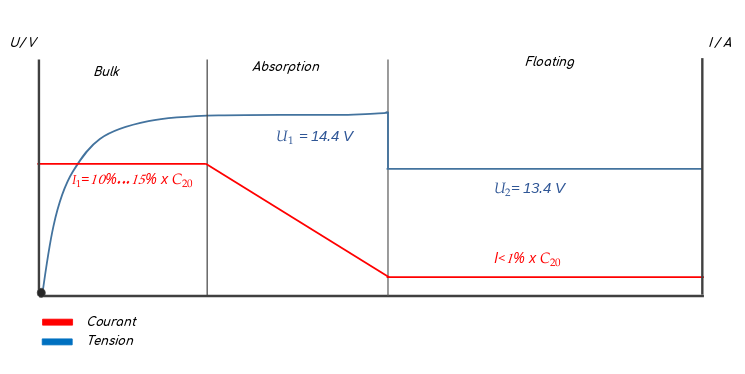
\includegraphics[width=16cm]{./img/ChargebatHumide.png}
	\caption{Les étapes de la tension de charge }
	\label{i1}
\end{figure}


\subsubsection{Le courant}

Le courant est la quantité de charge électrique qui circule à travers la batterie par unité de temps, mesurée en ampères (A). Plusieurs types de courants sont importants pour évaluer les performances et le comportement d'une batterie :

\begin{itemize}
	\item \textbf{Courant de charge (\(I_{\text{charge}}\))} : le courant appliqué à la batterie lors de son chargement. Il est souvent exprimé en fonction de la capacité nominale de la batterie (C), par exemple, un courant de charge de 0.1C pour une batterie de 100Ah serait de 10A.
	\item \textbf{Courant de décharge (\(I_{\text{discharge}}\))} : le courant que la batterie délivre lors de son utilisation. Comme pour le courant de charge, il est souvent exprimé en multiples de la capacité (C), par exemple, un courant de décharge de 0.5C pour une batterie de 100Ah serait de 50A.
	\item \textbf{Courant de pointe (\(I_{\text{peak}}\))} : le maximum de courant que la batterie peut fournir sur de courtes périodes sans subir de dommages. Ce paramètre est crucial pour des applications nécessitant des pics de puissance élevés.
	\item \textbf{Courant de repos (\(I_{\text{rest}}\))} : le courant minimal que la batterie délivre ou reçoit lorsqu'elle est en état de repos ou en charge très faible. Il est important pour évaluer les pertes internes de la batterie.
	\item \textbf{Courant de court-circuit (\(I_{\text{sc}}\))} : le courant maximal que la batterie peut fournir en cas de court-circuit. Il dépend de la résistance interne de la batterie et est un paramètre important pour la sécurité.
\end{itemize}

\subsubsection{La température}

Les températures extrêmes, qu'elles soient très élevées ou très basses, peuvent considérablement affecter le fonctionnement d'une batterie en service, influençant ainsi ses performances et d'autres paramètres critiques.

\subsubsection{La capacité}

\begin{itemize}
	\item \textbf{Capacité massique} : rapport entre l'énergie disponible d'une batterie ou cellule et son poids, exprimée en Wh/kg.
	\item \textbf{Capacité nominale (CN)} : valeur de la capacité indiquée par le fabricant pour des conditions d'opération spécifiques (température définie, courant et tension de coupure).
	\item \textbf{	C-rate (nC)} : mesure le courant de charge ou de décharge d'une batterie par rapport à sa capacité nominale. Une batterie évaluée à 1C fournit un courant égal à sa capacité en ampères pendant une heure. Par exemple, une batterie de 1000mAh à 1C fournit 1A pendant une heure, à 0.5C fournit 500mA pendant 2 heures, et à 2C fournit 2A pendant 30 minutes.
\end{itemize}

\subsubsection{Phénomène d'autodécharge}
L'autodécharge est la décomposition spontanée des matériaux actifs d'une cellule, entraînant une perte d'EMF due à une fuite interne de courant. Les batteries primaires sont les moins sujettes à l'autodécharge, suivies des batteries secondaires (rechargeables).

\begin{table}[h!]
	\centering
	\begin{tabular}{|>{\centering\arraybackslash}m{3cm}|>{\centering\arraybackslash}m{13cm}|}
		\hline
			\rule[0.5cm]{0cm}{0cm}\textbf{Type de batteries} & \textbf{Estimation de l'autodécharge} \\ \hline
			\rule[0.5cm]{0cm}{0cm}Primaire & 10\% en 5 ans\\ \hline
			\rule[0.5cm]{0cm}{0cm}Plomb-acide& 5\% par mois\\ \hline
		\rule[0.5cm]{0cm}{0cm}	Ni-Cd & 10-15\% en 24 heures, puis 10-15\% par 	\rule[0.5cm]{0cm}{0cm}mois \\ \hline
			\rule[0.5cm]{0cm}{0cm}Ni-MH & 30\% (avec faible résistance et grande capacité massique) \\ \hline
			\rule[0.5cm]{0cm}{0cm}Li-Ion& 5\% en 24 heures, puis 1-2\% /mois, >3\% pour les circuits de protection \\ \hline
	\end{tabular}
	\caption{Estimation de l'autodécharge pour différents types de batteries}
	\label{tab:autodecharge}
\end{table}

\newpage
\subsubsection{État de Charge (SoC)}
L'état de charge (SoC) d'une batterie représente l'énergie restante, influencé par des facteurs comme le courant et la température. Exprimé en pourcentage, 100\% indique une batterie pleine, et 0\% une batterie vide. Le SoC peut être déterminé par la méthode de comptage de Coulombs \cite{a1} \cite{a2} \cite{l2}.


\begin{equation}
\text{SoC}(t) = \text{SoC}(t-1) + \frac{1}{C_{\text{n}}} \int_{t-1}^{t} i(t) \, dt
\end{equation}

où :

\begin{itemize}
	\item \(\text{SoC}(t)\) est l'état de charge au temps \(t\),
	\item \(\text{SoC}(t-1)\) est l'état de charge au temps \(t-1\),
	\item \(i(\tau)\) est le courant mesuré à l'instant \(\tau\),
	\item \(C_{\text{n}}\) est la capacité nominale de la batterie en ampères-heures (Ah),
\end{itemize}

En pratique, la capacité actuelle (\(Q\)) peut être calculée à partir de la somme des produits du courant (\(I\)) et du temps (\(\Delta t\)) pour chaque intervalle de mesure :

\begin{equation}
Q = \int_{t_0}^{t} i(t) \, dt
\end{equation}

En pratique, cette intégration est souvent effectuée de manière discrète :

\begin{equation}
Q = \sum_{i=0}^{n} I_i \Delta t_i
\end{equation}

où :

\begin{itemize}
	\item \(I_i\) est le courant mesuré à l'intervalle \(i\),
	\item \(\Delta t_i\) est la durée de l'intervalle \(i\).
\end{itemize}

\subsubsection{La Profondeur de Décharge (DoD)}
La profondeur de décharge (DoD) indique la capacité retirée d'une batterie lors d'un cycle de décharge, exprimée en pourcentage par rapport à sa capacité maximale \cite{a2}. Par exemple, pour une batterie « YUASA 12V-24Ah », la DoD est calculée lorsque la batterie est déchargée avec un courant de 1,23A jusqu'à 12Ah de sa capacité C20.

\begin{equation}
\text{DoD} \% = \left( \frac{\text{Capacité retirée d'une batterie chargée (Ah)}}{C_x (\text{Ah})} \right) \times 100
\end{equation}

D'après cette équation  :

\[
\text{DoD} = \left( \frac{\text{Capacité initiale} - \text{Capacité retirée}}{C_{20}} \right) \times 100
\]

\[
\left( \frac{24\text{Ah} - 12\text{Ah}}{24\text{Ah}} \right) \times 100 = 50\%
\]

Selon ces équations , la profondeur de décharge est le complément de l'état de charge (SoC) :
\begin{equation}
\text{DoD} \% = (1 - \text{SoC}) \times 100
\end{equation}

Ce paramètre est crucial pour le dimensionnement correct d'une batterie. Identifier précisément la DoD permet de gérer efficacement la durée de vie et la performance de la batterie.

\subsubsection{Le Nombre de Cycles (Nb\_Cycles)}
Le nombre de cycles (Nb\_Cycles) correspond au nombre de cycles charge/décharge qu'une batterie peut effectuer tout en maintenant sa tension de coupure au-dessus de V\textsubscript{Cut-Off}. Il dépend de la profondeur de décharge (DoD) et est généralement fourni par le fabricant, mais peut être déterminé après des tests spécifiques. Ce paramètre influence la durée de vie et la performance de la batterie.

\subsubsection{L’état de santé (SOH)}
L’état de santé (SOH) mesure la capacité de la batterie à fournir les performances spécifiées par rapport à une batterie neuve. Il permet d’estimer la durée de vie restante (Nb\_Cycles) et suit la dégradation des performances \cite{a2}.


\begin{equation}
\text{SOH} \% = \left( \frac{\text{Capacité d'une batterie utilisée (Ah)}}{C_x (\text{Ah})} \right) \times 100
\end{equation}

Pour certaines prédéfinitions, la batterie est considérée en fin de vie (EOL) lorsqu'elle atteint un SOH de 80\%. Cela signifie que lorsqu'une batterie ne peut plus fournir que 80\% de sa capacité nominale, elle doit être remplacée ou reconditionnée pour continuer à garantir des performances optimales.

\subsection{Structure de la batterie}
Une batterie est constituée de plusieurs cellules électrochimiques assemblées en structures prismatiques, cylindriques, etc. Ces cellules forment la batterie, définissant sa tension, son courant, et sa durée de vie, selon les normes ou l'application.


\begin{figure}[H]
	\centering
	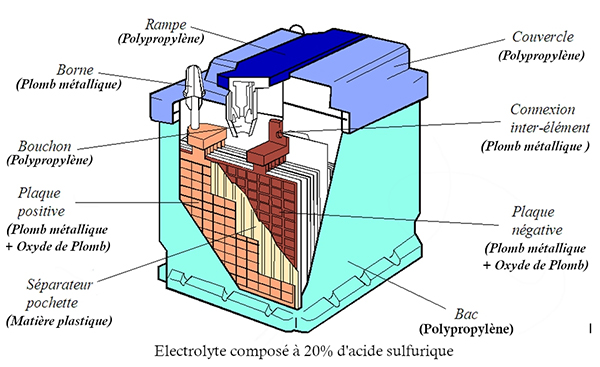
\includegraphics[width=13cm]{./img/stricture1.jpg}
	\caption{Structure d'une batterie}
	\label{i1}
\end{figure}
\subsection{Les batteries solaires}

Les batteries solaires stockent l'énergie produite par les panneaux photovoltaïques. Elles sont essentielles pour les systèmes autonomes, car les panneaux ne génèrent de l'électricité que durant la journée. Les batteries permettent d'utiliser l'électricité stockée pendant la nuit ou par temps nuageux.

\subsubsection{Fonctionnement d’une batterie solaire}

Les batteries solaires stockent l'énergie sous forme chimique et la libèrent via des réactions internes. Conçues pour des décharges lentes et des recharges espacées, elles accumulent plus d’énergie que les batteries de voiture ou d’appareils électroniques.


\subsection{Types de Batteries Solaires}

Les batteries solaires se classifient en plusieurs types, chacun ayant ses caractéristiques spécifiques. Voici les principales catégories \cite{a3} \cite{a4} :

\begin{table}[h!]
	\centering
	\begin{tabular}{|>{\centering\arraybackslash}m{5cm}|>{\centering\arraybackslash}m{10cm}|}
		\hline
		\textbf{Type de Batterie} & \textbf{Exemples} \\ \hline
		\rule[0.5cm]{0cm}{0cm} \textbf{Batteries au Plomb} & Plomb Acide Liquide (Inondées ou Plomb Ouvert), AGM, Gel \\ \hline
		\rule[0.5cm]{0cm}{0cm} \textbf{Batteries au Lithium} & Lithium-Ion, LiFePO4, LiMn2O4 \\ \hline
		\rule[0.5cm]{0cm}{0cm} \textbf{Autres Technologies} & Batteries à Flux (Redox), Batteries à Électrolyte Solide, Batteries Zinc-Air, Batteries Aluminium-Air \\ \hline
	\end{tabular}
	\caption{Types de batteries et leurs exemples}
\end{table}
	

Bien que d'autres types de batteries existent, ceux mentionnés ci-dessus sont fréquemment utilisés et disponibles sur le marché.

Chaque type de batterie a ses propres tensions de charge et décharge spécifiques. Examinons les tensions de charge pour différentes batteries ayant une tension nominale de 12V :


\begin{table}[h!]
	\centering
	\begin{tabular}{|>{\centering\arraybackslash}m{5cm}|>{\centering\arraybackslash}m{5cm}|>{\centering\arraybackslash}m{5cm}|}
		\hline
			\rule[0.5cm]{0cm}{0cm}\textbf{Type de Batterie} &	\rule[0.5cm]{0cm}{0cm} \textbf{Tension de Charge Maximale} & \textbf{Tension de Décharge Minimale} \\ \hline

			\rule[0.5cm]{0cm}{0cm}\quad  Plomb Acide  & 14.4V - 14.8V & 10.5V \\ \hline
			\rule[0.5cm]{0cm}{0cm}\quad  AGM  & 14.4V - 14.6V & 10.5V \\ \hline
			\rule[0.5cm]{0cm}{0cm}\quad   Gel & 14.2V - 14.4V & 10.5V \\ \hline
	
		\rule[0.5cm]{0cm}{0cm}	\quad  Lithium-Ion & 4.2V par cellule & 2.5V - 3.0V par cellule \\ \hline
		\rule[0.5cm]{0cm}{0cm}	\quad  LiFePO4 & 3.6V - 3.65V par cellule & 2.0V - 2.5V par cellule \\ \hline
			\rule[0.5cm]{0cm}{0cm}\quad  LiMn2O4 & 4.2V par cellule & 2.5V - 3.0V par cellule \\ \hline
	\end{tabular}
	\caption{Tensions de charge maximales et de décharge minimales}
\end{table}



\subsubsection{Comparaison des Types de Batteries Solaires}

Le tableau ci-dessous présente une comparaison des différents types de batteries solaires, mettant en évidence leurs caractéristiques distinctes et leurs différences :

\begin{landscape}
	\begin{table}[h!]
		\centering
		\caption{Comparaison des différents types de batteries solaires}\vspace{0.3cm}
		\begin{tabular}{|>{\centering\arraybackslash}m{3cm}|>{\centering\arraybackslash}m{1.5cm}|>{\centering\arraybackslash}m{1.5cm}|>{\centering\arraybackslash}m{3cm}|>{\centering\arraybackslash}m{2cm}|>{\centering\arraybackslash}m{5cm}|>{\centering\arraybackslash}m{3cm}|>{\centering\arraybackslash}m{1.5cm}|}
			\hline
				\rule[0.5cm]{0cm}{0cm}\textbf{Type de Batterie} & \textbf{Cycles de Vie} & \textbf{DoD (\%)} & \textbf{Matériaux} & \textbf{Prix} & \textbf{Impact Environnemental} & \textbf{Température (\textdegree C)} & \textbf{Volume} \\
			\hline
			Plomb Acide Liquide & 500-1000 & 50-70 & Plomb, acide sulfurique & Moins cher & Pollution par le plomb, recyclage possible, dégage de l'hydrogène & -20 à 50 & Grand \\
			\hline
			AGM  & 600-1200 & 60-80 & Plomb, acide sulfurique & Moins cher & Pollution par le plomb, recyclage possible, dégage de l'hydrogène & -20 à 50 & Moyen \\
			\hline
			Gel & 700-1400 & 60-80 & Plomb, électrolyte gélifié & Modéré & Pollution par le plomb, recyclage possible, dégage de l'hydrogène & -20 à 50 & Moyen \\
			\hline
			Lithium-Ion & 2000-5000 & 80-90 & Lithium, cobalt, nickel & Cher & Extraction de lithium, recyclage complexe, dégage de la chaleur & -20 à 60 & Petit \\
			\hline
			Lithium-Fer-Phosphate (LiFePO4) & 3000-7000 & 80-90 & Lithium, fer, phosphate & Modéré & Impact moindre, recyclage possible, dégage de la chaleur & -20 à 60 & Petit \\
			\hline
			Lithium-Manganèse (LiMn2O4) & 1000-2000 & 80-90 & Lithium, manganèse & Modéré & Extraction de lithium et manganèse, recyclage complexe, dégage de la chaleur & -20 à 60 & Petit \\
			\hline
			Batteries à Flux (Redox) & 5000-10000 & 100 & Vanadium, électrolytes liquides & Modéré & Impact limité, électrolytes recyclables, peut dégrader l'environnement aqueux & -10 à 40 & Très grand \\
			\hline
			Batteries à Électrolyte Solide & 1000-5000 & 80-90 & Matériaux solides, lithium & Cher & Impact limité, recyclage complexe, dégage de la chaleur & -20 à 60 & Petit à moyen \\
			\hline
			Batteries Zinc-Air & 200-500 & 100 & Zinc, air & Moins cher & Impact faible, recyclable, dégage de l'oxygène & -20 à 50 & Moyen \\
			\hline
			Batteries Aluminium-Air & 200-500 & 100 & Aluminium, air & Moins cher & Impact faible, recyclable, dégage de l'oxygène & -20 à 50 & Moyen à grand \\
			\hline
		\end{tabular}
	\end{table}
\end{landscape}

%\subsection{Réactions chimiques pendant la charge et décharge}
%Comprendre les phénomènes chimiques fondamentaux est crucial pour appréhender le fonctionnement des batteries. Nous allons examiner les réactions chimiques typiques qui se produisent pendant la charge et la décharge dans deux types de batteries : les batteries au plomb et les batteries au lithium \cite{t1}.
%
%\subsubsection{La batterie au Plomb-Acide}
%
%La batterie au plomb-acide est une technologie largement éprouvée et presque entièrement recyclable. Elle se distingue par son coût relativement bas par rapport aux autres types de batteries, ce qui en fait une référence pour comparer les performances des autres technologies. Son principe de fonctionnement repose sur une réaction d'oxydoréduction caractéristique :
%
%\[
%\text{PbO}_2 + \text{Pb} + 2 \text{H}_2\text{SO}_4 \rightleftharpoons 2 \text{PbSO}_4 + 2 \text{H}_2\text{O}
%\]
%
%Ici, \(\text{PbO}_2\) est l'électrode positive (+) et \(\text{Pb}\) est l'électrode négative (-). L'électrolyte utilisé est l'acide sulfurique (\(\text{H}_2\text{SO}_4\)).\\
%
%\textbf{Processus de décharge :}
%Pendant la décharge, le plomb à l'anode s'oxyde en perdant deux électrons, tandis que le plomb à la cathode se réduit en gagnant deux électrons. L'hydrogène et l'oxygène formés se combinent pour créer de l'eau (\(\text{H}_2\text{O}\)).
%	\begin{align*}
%	\textbf{Anode (-)} &: \text{Pb} + \text{H}_2\text{SO}_4 \rightarrow \text{PbSO}_4 + 2 \text{H}^+ + 2 e^-\\
%	\textbf{Cathode (+) }&:\text{PbO}_2 + \text{H}_2\text{SO}_4 + 2 e^- \rightarrow \text{PbSO}_4 + 2 \text{OH}^-\\
%	\textbf{Cellule} &:\text{PbO}_2 + \text{Pb} + 2 \text{H}_2\text{SO}_4 \rightleftharpoons 2 \text{PbSO}_4 + 2 \text{H}_2\text{O}
%	\end{align*}
%
%
%\textbf{Processus de charge :}
%Lors de la charge, les réactions inverses de celles de la décharge se produisent, car ces réactions sont réversibles. L'eau est décomposée aux électrodes, l'oxygène réagit avec le plomb à l'électrode positive, tandis que l'hydrogène réagit avec l'acide à l'électrode négative.
%\begin{align*}
%	\textbf{Anode (+)} & : \text{Pb}^{2+} + 2 \text{H}_2\text{O} \rightarrow \text{PbO}_2 + 4 \text{H}^+ + 2 e^- \\
%	\textbf{Cathode (-)} &: \text{PbSO}_4 + 2 e^- \rightarrow \text{Pb} + \text{SO}_4^{2-} \\
%	\textbf{Cellule} &:\text{Pb}^{2+} + 2 \text{H}_2\text{O} \rightleftharpoons \text{PbO}_2 + \text{Pb} + 4 \text{H}^+ 
%\end{align*}
%
%
%\subsubsection{La batterie lithium-ion (Li-Ion) :}
%Grâce à ses caractéristiques attrayantes, comme la légèreté du lithium (6,94 g/mol) et sa densité énergétique élevée (3860 mAh/g), cette technologie a été étudiée depuis les années 1950. Les premières batteries commerciales Li-Ion sont apparues dans les années 1990. Aujourd'hui, les types les plus courants sont les Lithium-Ion (Li-Ion) et Lithium-Polymères (Li-Po).
%
%\textbf{Processus de décharge} :
%Pendant la décharge, les ions lithium (\(\text{Li}^+\)) se déplacent de l'anode (négative) vers l'électrolyte, tandis que les électrons (\(e^-\)) circulent dans le circuit externe pour fournir de l'énergie. À la cathode (positive), les ions lithium et les électrons réagissent avec \(\text{Li}_{1-x}\text{CoO}_2\) pour former \(\text{LiCoO}_2\). Cette réaction maintient l'équilibre entre les états chargés et déchargés des matériaux actifs.
%\begin{align*}
%\text{Anode (-)} & : \text{Li}_x\text{C} \rightarrow \text{C} + x \text{Li}^+ + x e^-  \\
%\text{Cathode (+)} & : \text{Li}_{1-x}\text{CoO}_2 + x \text{Li}^+ + x e^- \rightarrow \text{LiCoO}_2 \\
%\text{CELLULE} & : \text{Li}_{1-x}\text{CoO}_2 + \text{Li}_x\text{C} \leftrightarrows \text{C} + \text{LiCoO}_2 
%\end{align*}
%
%\textbf{Processus de charge} :
%es électrons (\(e^-\)) sont extraits de l'anode (positive) par une source d'alimentation externe et passent par le circuit externe. Simultanément, les ions lithium (\(\text{Li}^+\)) migrent de la cathode (négative) vers l'anode à travers l'électrolyte. À l'anode, les ions lithium se réintègrent dans le graphite pour reformer \(\text{Li}_x\text{C}\). À la cathode, les électrons et les ions lithium réagissent pour reformer \(\text{Li}_{1-x}\text{CoO}_2\). Ce processus recharge les matériaux actifs de la batterie.
%\begin{align*}
%\text{Anode (+)} & : \text{LiCoO}_2 \rightarrow \text{Li}_{1-x}\text{CoO}_2 + x \text{Li}^+ + x e^-  \\
%\text{Cathode (-)} & : \text{C} + x \text{Li}^+ + x e^- \rightarrow \text{Li}_x\text{C}  \\
%\text{CELLULE} & : \text{Li}_{1-x}\text{CoO}_2 + \text{Li}_x\text{C} \leftrightarrows \text{C} + \text{LiCoO}_2 
%\end{align*}

\section{Procédure de dimensionnement d’une champ photovoltaïque }
La conception d'une installation photovoltaïque autonome est un processus assez complexe en raison des nombreux paramètres à prendre en compte.

\subsection{Besoin énergétique des applications}

Pour dimensionner correctement un système, il est crucial d'évaluer les besoins énergétiques des applications à alimenter, ce qui se traduit par la puissance nécessaire. La relation entre puissance et énergie, deux grandeurs liées par le temps, est donnée par :
\begin{figure}[H]
	\centering
	\begin{subfigure}{0.40\textwidth} % Largeur de la partie formule
		\centering
		\begin{equation}
		E = P \times t
		\end{equation}
	\end{subfigure}
	\hfill
	\begin{subfigure}{0.55\textwidth} % Largeur de la partie explication
		\centering
		\begin{itemize}
			\item \( E \) : énergie (en Wh/j),
			\item \( P \) : puissance (en Watts),
			\item \( t \) : temps d’utilisation (en heures).
		\end{itemize}
	\end{subfigure}
\end{figure}


Cette formule permet de calculer le besoin énergétique journalier d'une application, en multipliant la puissance consommée par la durée d’utilisation quotidienne.

\subsection{Énergie solaire récupérable}

\subsubsection{Inclinaison et orientation des panneaux}  
L'orientation et l'inclinaison des panneaux influencent directement leur rendement. Pour maximiser la production, ils doivent être orientés vers l'équateur (sud dans l'hémisphère nord, nord dans l'hémisphère sud) et inclinés selon la période la moins ensoleillée.  

\subsubsection{Données météorologiques}  
Le dimensionnement photovoltaïque dépend du rayonnement solaire local : plus il est élevé, moins il faut de panneaux pour un besoin donné.

\subsection{Énergie produite (Wh/jour)}

L'énergie à produire par le champ photovoltaïque est calculée selon la formule suivante :

\begin{equation}
Ep \, (\text{Wh}) = \frac{Ec}{k}
\end{equation}

Où :

\begin{itemize}
	\item \textbf{Ep} : Énergie à produire par le champ photovoltaïque en Wh/jour
	\item \textbf{Ec} : Énergie totale consommée en Wh/jour
\item \textbf{k} : Facteur de correction tenant compte des incertitudes météorologiques, du rendement des modules, des batteries, du régulateur, de l'onduleur et des pertes dans les câbles. Il varie entre 0,55 et 0,75.

\end{itemize}

\subsection{Puissance crête (Pc) des modules photovoltaïques}

La puissance crête totale du champ photovoltaïque dépend de l'irradiation quotidienne du lieu d'utilisation. Elle est donnée par :

\begin{equation}
Pc = \frac{Ep}{Ir}
\end{equation}
Où :

\begin{itemize}
	\item \textbf{Pc} : Puissance crête totale des modules photovoltaïques en W
	\item \textbf{Ep} : Énergie à produire par le champ photovoltaïque en Wh/jour
	\item \textbf{Ir} : Irradiation journalière du mois le plus défavorable en kWh/m²/jour
\end{itemize}

\subsection{Choix de la tension de fonctionnement}

Le choix de la tension de fonctionnement d'un système dépend de la disponibilité du matériel, ainsi que des niveaux de puissance et d'énergie nécessaires selon le type d'application. Le tableau suivant montre les tensions du système correspondant à chaque intervalle de puissance crête :

\begin{table}[H]
	\centering
	\begin{tabular}{|c|c|c|c|c|}
		\hline
			\rule[0.5cm]{0cm}{0cm}\textbf{Puissance du Champ (Wc)} & 0-500 Wc & 500 Wc - 2 kWc  & 2 - 10 kWc & 	> 10 kWc \\
		\hline
			\rule[0.5cm]{0cm}{0cm}\textbf{Tension Recommandée (V DC)} & 12 V  & 24 V & 48 V & > 48 V \\
		\hline
	\end{tabular}
\caption{Tension recommandée pour les systèmes photovoltaïques}
\end{table}

\subsubsection{Choix du type de module photovoltaïque}

Le choix du type de module dépend de plusieurs facteurs : la tension de fonctionnement choisie, la puissance maximale, le courant de court-circuit (Icc), le dimensionnement, et le prix.

\subsubsection{Détermination du nombre de modules à installer}

À partir de la puissance crête des panneaux, le nombre de panneaux solaires nécessaires à l'installation est déterminé par la formule :

\begin{equation}
Np = \frac{Pc}{Ppv}
\end{equation}


Où :

\begin{itemize}
	\item \textbf{Np} : Nombre de panneaux nécessaires
	\item \textbf{Pc} : Puissance crête totale des modules photovoltaïques en W
	\item \textbf{Ppv} : Puissance crête d’un module photovoltaïque en W
\end{itemize}

\subsubsection{Répartition des modules}

Le choix de la tension du générateur PV est étroitement lié à la puissance crête demandée. 
\textbf{Nombre de panneaux en série et en parallèle}\\

\textbf{Nombre de panneaux en série} :
	\begin{equation}
N_s = \frac{U}{U_n}
\end{equation}
Où :
	\begin{itemize}
	\item \textbf{U} : Tension du système,
	\item \textbf{U\textsubscript{n}} : Tension nominale d'un module.
\end{itemize}


\textbf{Nombre de branches en parallèle} :

	\begin{equation}
N_{bp} = \frac{N_{mb}}{N_s}
\end{equation}
Où : 

	\begin{itemize}
	\item \textbf{Nmb} : Nombre total de modules,
	\item \textbf{Ns} : Nombre de panneaux en série.
\end{itemize}


\subsection{Caractéristiques du générateur}

\textbf{Puissance crête d’un champ} :

	\begin{equation}
Pc/champ = N_{bp} \times N_s \times P_{cm}
\end{equation}

Où :
	\begin{itemize}
	\item \textbf{Pcm} : Puissance crête d’un module,
	\item \textbf{Nbp} : Nombre de branches parallèles,
	\item \textbf{Ns} : Nombre de panneaux en série.
\end{itemize}

\textbf{Surface occupée par le générateur} :
	\begin{equation}
St = Sm \times Nm
\end{equation}
Où :
	\begin{itemize}
	\item \textbf{Sm} : Surface d’un module,
	\item \textbf{Nm} : Nombre de modules.
\end{itemize}


\subsection{Dimensionnement des éléments de stockage}

La capacité nominale des batteries est donnée par l’expression :


\begin{equation}
Cu = \frac{Cj \times Nj}{U \times Pd}
\end{equation}
Où :\begin{itemize}
	\item \textbf{Cj} : Capacité journalière requise par champ (en Ah/jour)
	\item \textbf{Nj} : Nombre de jours d'autonomie
	\item \textbf{Pd} : Profondeur de décharge (par exemple, 0.8 pour 80\%).
	\item \textbf{U} : Tension du système (en volts, V)
\end{itemize}
La Capacité Journalière est donnée par :
	\begin{equation}
C_j = \frac{E_j}{U}
\end{equation}


\textbf{Où :}

\begin{itemize}
	\item $C_j$ : Capacité journalière requise par champ (en Ah/jour)
	\item $E_j$ : Énergie journalière nécessaire (en watt-heures, Wh/jour)
	\item $U$ : Tension du système (en volts, V)
\end{itemize}


Autonomie souhaitée pour l'installation : 

\begin{equation}
Estockage = Ep \times Nj
\end{equation}
Où :

\begin{itemize}
	\item \textbf{Estockage} : Énergie de stocker 
	\item \textbf{Nj} : Nombre de jours d'autonomie

\end{itemize}

On détermine le nombre des batteries nécessaire en utilisant les formule suivantes : 
\textbf{Nombre de batteries en série} :
\begin{equation}
N_s = \frac{V_{module}}{V_{batterie}} 
\end{equation}


\textbf{Nombre de chaînes en parallèle} : 

	\begin{equation}
N_p = \frac{Cu}{Cn}
\end{equation}
Où :
	\begin{itemize}
	\item \textbf{Cu} : Capacité totale requise des batteries,
	\item \textbf{Cn} : Capacité nominale d'une seule batterie.
\end{itemize}

\textbf{Nombre total de batteries} :
	\begin{equation}
N_t = N_s \times N_p 
\end{equation}




\subsection{Dimensionnement du régulateur}

Le régulateur contrôle les flux d’énergie et protège la batterie contre les surcharges et décharges profondes. Le régulateur sera dimensionné d’après la tension et le courant d’entrée :

\begin{equation}
Imax = \frac{Pc/champ}{U}
\end{equation}
\subsection{Dimensionnement de l’onduleur}
L'onduleur convertit le courant continu en courant alternatif. Son dimensionnement se base sur la somme des puissances maximales des équipements à alimenter, en tenant compte des courants de pointe élevés et du facteur de puissance (cos \(\theta\)). La puissance apparente (S) est calculée par :

	\begin{equation}
S^2 = P^2 + Q^2
\end{equation}
Où :
	\begin{itemize}
	\item \textbf{P} : Puissance active,
	\item \textbf{Q} : Puissance réactive.
\end{itemize}

\subsection{Choix des câbles}

Les câbles solaires doivent résister aux conditions spéciales liées à leur utilisation. La résistance d’un câble dépend de la résistivité des matériaux, de la longueur du câble, de la section et de la température.

\begin{equation}
R = \frac{\rho \cdot L}{S}
\end{equation}
Où :
	\begin{itemize}
	\item \textbf{R} : Résistance (\(\Omega\)),
	\item \textbf{\(\rho\)} : Résistivité (\(\Omega \cdot\)m),
	\item \textbf{L} : Longueur du câble (m),
	\item \textbf{S} : Section du câble (m²).
\end{itemize}



\subsubsection{Calcul de la section des câbles}

\textbf{Courant de Sortie d’un Panneau} :

	\begin{equation}
I = \frac{P}{U}
\end{equation}
Où :
	\begin{itemize}
	\item \textbf{I} : Courant de sortie d’un panneau en ampère (A),
	\item \textbf{P} : Puissance d’un panneau en watt (W),
	\item \textbf{U} : Tension nominale d’un panneau en volt (V).
\end{itemize}

\textbf{Section des conducteurs entre les panneaux et le boîtier de raccordement} :

\begin{align*}
\Delta U &= U \cdot 0{,}02 & \quad R &= \frac{\Delta U}{I} & \quad S &= \frac{\rho \cdot L}{R}
\end{align*}
\subsection{Courant circulant entre les batteries et l’onduleur}

\textbf{Puissance crête du champ photovoltaïque} :
\begin{align}
Pc &= N \times P & \quad I &= \frac{Pc}{U}
\end{align}


\textbf{Courant circulant entre les batteries et l’onduleur à la puissance nominale} :

\begin{equation}
Imax \, batteries = \frac{P \, max \, onduleur}{U \, batterie}
\end{equation}

\section{Conclusion}
Nous avons étudié les diverses applications des systèmes photovoltaïques et constaté que leur performance dépend de plusieurs facteurs, tels que la qualité des panneaux solaires, des batteries, et des autres équipements utilisés, ainsi que du dimensionnement adéquat du système. Le bon fonctionnement d'une batterie dépend de plusieurs paramètres, notamment la température, la tension et le courant, ce qui nécessite une surveillance régulière afin de garantir des performances optimales.

Dans le chapitre suivant, nous traiterons du fonctionnement des dispositifs de surveillance de ces accumulateurs, indispensables pour optimiser la gestion et la performance des installations photovoltaïques.







